\documentclass[11pt,twoside]{article}

\usepackage{amsmath}
\usepackage{amssymb}
\usepackage{amsthm}
\usepackage{courier} % Required for the courier font
\usepackage{extramarks} % Required for headers and footers
\usepackage{fancyhdr} % Required for custom headers
\usepackage{graphicx} % Required to insert images
\usepackage{lastpage} % Required to determine the last page for the footer
\usepackage{listings} % Required for insertion of code
\usepackage{lipsum} % Used for inserting dummy 'Lorem ipsum' text into the template
\usepackage{mathtools}
\usepackage{subcaption}

\usepackage[margin=1in]{geometry}
\usepackage[usenames,dvipsnames]{color} % Required for custom colors

\usepackage{color}

\definecolor{mygreen}{rgb}{0,0.6,0}
\definecolor{mygray}{rgb}{0.5,0.5,0.5}
\definecolor{mymauve}{rgb}{0.58,0,0.82}

\lstset{ %
  commentstyle=\color{mygreen},    % comment style
  frame=single,	                   % adds a frame around the code
  keywordstyle=\color{blue},       % keyword style
  language=Python,                 % the language of the code
  numbers=left,                    % where to put the line-numbers; possible values are (none, left, right)
  numbersep=5pt,                   % how far the line-numbers are from the code
  numberstyle=\tiny\color{mygray}, % the style that is used for the line-numbers
  stringstyle=\color{mymauve},     % string literal style
}

\begin{document}

\title{CSC411 - Project \#4}
\author{Yui Chit (Michael) Wong - 999806232\\Yijin (Catherine) Wang - 998350476}
\maketitle

\clearpage

\section*{Part 1}
\paragraph{Question}
Explain precisely why the code corresponds to the pseudocode below. Specifically, in your report, explain how all the terms ( $G_t$ , $\pi$ , and the update to $\theta$ ) are computed, quoting the relevant lines of Python.

\begin{figure*}[h]
	\centering
	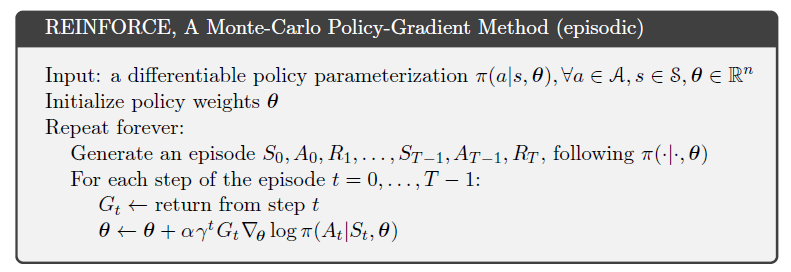
\includegraphics[scale=0.8]{sutton&barto.png}
	\caption*{Pseudocode}
\end{figure*}

\paragraph{Answer}
As mentioned on the assignment page, the policy function $\pi_{\theta}$ is implemented with a single-hidden-layer of neural network. Since the actions for the bipedal walker is continuous, we have to use a Gaussian distribution on $\pi$. Thus we pass the hidden layer into two separately fully connected output, which represents the $\mu$ and $\sigma$ to the normal distribution. The activation function are $tanh$ and $softplus$ (variation on $ReLU$) respectively. The $sigma$ value are also clipped if it is too small or big.

\begin{lstlisting}
# 1 layer of hidden unit. Activation is ReLU
hidden = fully_connected(
    inputs=x,
    num_outputs=hidden_size,
    activation_fn=tf.nn.relu,
    weights_initializer=hw_init,
    weights_regularizer=None,
    biases_initializer=hb_init,
    scope='hidden')

# use last layer of neural network as phi(a, s) (the feature)
# mu = phi(s, a)^T dot theta
mus = fully_connected(
    inputs=hidden,
    num_outputs=output_units,
    activation_fn=tf.tanh,
    weights_initializer=mw_init,
    weights_regularizer=None,
    biases_initializer=mb_init,
    scope='mus')

# softplus is similar to ReLU. Activation function is g(x) = ln(1+e^x)
sigmas = tf.clip_by_value(fully_connected(
    inputs=hidden,
    num_outputs=output_units,
    activation_fn=tf.nn.softplus,
    weights_initializer=sw_init,
    weights_regularizer=None,
    biases_initializer=sb_init,
    scope='sigmas'),
    TINY, 5)
\end{lstlisting}

As for the weight intialization, if there is no weight saved from the previous run, we will initialize the weight $\theta$. There are one $w$ and $b$ for each of the layers (hidden, $\mu$, $\sigma$). When initializing the weight to each layer, the program uses $xavier initialization$, another variation of random weight initialization that keep the scale of the gradients in roughly the same scale.

\begin{lstlisting}
# if we have the w's and b's saved, load it. Otherwise initialize it
if args.load_model:
    model = np.load(args.load_model)
    hw_init = tf.constant_initializer(model['hidden/weights'])
    hb_init = tf.constant_initializer(model['hidden/biases'])
    mw_init = tf.constant_initializer(model['mus/weights'])
    mb_init = tf.constant_initializer(model['mus/biases'])
    sw_init = tf.constant_initializer(model['sigmas/weights'])
    sb_init = tf.constant_initializer(model['sigmas/biases'])
else:
    hw_init = weights_init
    hb_init = relu_init
    mw_init = weights_init
    mb_init = relu_init
    sw_init = weights_init
    sb_init = relu_init
\end{lstlisting}

Once everything is initialized, we will start training. For each iteration, we will reset the environment (line 2), then generate the states, actions, and rewards from time 0 to time $T$. When generating the actions, we will randomly sample from the $\pi$ normal distribution (line 16). Then based on the $pi.sample()$, we will generate the corresponding action $pi_sample$, and using the action, the new state, reward would be generated. We will keep track of all the states, actions, and rewards in 3 lists ($ep\_states, ep\_actions, $ and $ep\_rewards$). We will also keep track of the total discounted rewards using the variable $G$ (line 20). Then to obtain $G_t$, the discounted reward starting from time t, the program calls a culmulation sum function on the $ep_rewards$ then subtract it from $G$ (line 30). Thus $returns$ would be storing the total discouned rewards for each time from time 0 to $T-1$.

\begin{lstlisting}
for ep in range(16384):
    obs = env.reset()	# reset the environment

    G = 0	    # generating all the states and actions and rewards
    ep_states = []
    ep_actions = []
    ep_rewards = [0]
    done = False
    t = 0
    I = 1
    while not done:
        ep_states.append(obs)
        env.render()
        # pi.sample() is the list of randomly generated probablity
        # pi_sample becomes the action
        action = sess.run([pi_sample], feed_dict={x:[obs]})[0][0]
        ep_actions.append(action)
        obs, reward, done, info = env.step(action)
        ep_rewards.append(reward * I)
        G += reward * I # G is the total discounted reward
        I *= gamma

        t += 1
        if t >= MAX_STEPS:
            break
    # done generating

    if not args.load_model:
        # G_t = total - culmulative up to time t. 
        returns = np.array([G - np.cumsum(ep_rewards[:-1])]).T
        index = ep % MEMORY
        
        # ep_states contains all the state S_0 to S_T-1
        # ep_actions contains all the actions from A_0 to A_T-1
        # returns (ie reward) contains all the G_t's form t=0 to t=T
        _ = sess.run([train_op],
                    feed_dict={x:np.array(ep_states),
                                y:np.array(ep_actions),
                                Returns:returns })
\end{lstlisting}

Then we will pass the list of states, actions, and the returns into the training step (line 36-39). Then tensorflow will use the state and the weights to generate a new $\mu$ and $\sigma$. Then it will compute the log probability of the actions given the generate $\mu$ and $\sigma$. 

\begin{lstlisting}
# log probability of y given mu and sigma
log_pi = pi.log_prob(y, name='log_pi')
\end{lstlisting}

The cost function used is $J(\theta) = -\sum[G_t log \pi (A_t | S_t, \theta)]$. The program uses gradient descent to adjust the $\theta$ to minimize the cost function

\begin{lstlisting}
# Returns is a 1 x (T-1) array for float (rewards)
Returns = tf.placeholder(tf.float32, name='Returns')
optimizer = tf.train.GradientDescentOptimizer(alpha)
train_op = optimizer.minimize(-1.0 * Returns * log_pi)
\end{lstlisting}

\clearpage



\section*{Part 2}

\paragraph{Question}
Your job is to now write an implementation of REINFORCE that will run for the CartPole-v0 (source code here ) environment.

In the Cart Pole task, two actions are possible – applying a force pushing left, and applying a force pushing right. Each episode stops when the pole inclides at an angle that larger than a threshold, or when the cart moves out of the frame. The at each time-step before the episode stops, the reward is 1.

The policy function should have two outputs – the probability of “left” and the probability of “right.’ Implement the policy function as a softmax layer (i.e., a linear layer that is then passed through softmax.) Note that a softmax layer is simply a fully-connected layer with a softmax actication.

In your report, detail all the modifications that you had to make to the handout code, one-by-one, and briefly state why and how you made the modifications. Include new code (up to a few lines per modification) that you wrote in your report.

\paragraph{Answer}

The modifications we made are:
\begin{enumerate}
\item We changed the network model.\\
In part 1, the network has a hidden layer which computes the feature vector of $x$, and pass the feature vector to one layer that computes $\mu$, and another layer that computes $\sigma$, then use the output of $\mu$ and $\sigma$ to generate $\pi$ and use the $\pi$ to generate action.\\
Our network for part 2 is simpler, we don't have a hidden layer. We just have a fully connected layer that takes $x$ as input, and output two output units. Then we use sigmoid as the activation function on the output to make the output in range of (0, 1), and then pass the output from activation function to softmax. The output of softmax is a size 2 vector that each element indicates the probability of an action.\\
Therefore, we removed the setup of layers we don't need, and built our network as follows. (We also adjusted the value of $\alpha$ and $\gamma$.)
\begin{lstlisting}
alpha = 1e-6
gamma = 0.99

try:
    output_units = env.action_space.shape[0]
except AttributeError:
    output_units = env.action_space.n

input_shape = env.observation_space.shape[0]
w = tf.get_variable("w", shape=[input_shape, output_units])
b = tf.get_variable("b", shape=[output_units])
x = tf.placeholder(tf.float32, shape=(None, input_shape), name='x')
y = tf.placeholder(tf.int32, shape=(None, 1), name='y')

layer1 = tf.sigmoid(tf.matmul(x, w)+b)
soft_max = tf.nn.softmax(layer1)
\end{lstlisting}

\item Since we have bernoulli distribution instead of the normal distribution used in part 1 for $\pi$, our $\pi$ is the output of softmax. Our $pi\_sample$ gets the action of higher corresponding probability from softmax. Out $log\_pi$ is the logarithm of softmax. And we use $act\_pi$ instead of $log\_pi$ to calculate the cost. We used the line of code which is provided to us to compute $act\_pi$. The code converts $y$ which is a list of actions of shape $n \times 1$ to the one hot encoding matrix which has shape $n \times 2 \times 1$, where $n$ is the number of states. The code also add one more dimension to $log\_pi$ which converts the shape of $log\_pi$ from $n \times 2$ to $n \times 1 \times 2$. The result of multiplication of the two converted matrices is a $n \times 1 \times 1$ matrix which is a list of log probabilities of corresponding actions.\\
Then we used the $act\_pi$ to compute the cost.

\begin{lstlisting}
pi_sample = tf.argmax(soft_max, axis=1)
log_pi = tf.log(soft_max)
act_pi = tf.matmul(tf.expand_dims(log_pi, 1), tf.one_hot(y, 2, axis=1))

Returns = tf.placeholder(tf.float32, name='Returns')
optimizer = tf.train.GradientDescentOptimizer(alpha)
train_op = optimizer.minimize(-1.0 * Returns * act_pi)
\end{lstlisting}

The rest of the code are mostly what we got from part 1.

\end{enumerate}

\clearpage



\section*{Part 3}
Train CartPole using your implementation of REINFORCE. (Use a very small learning rate, and a discount rate $\gamma=0.99$.) You do not have to train it until it works perfectly (i.e., the episode doesn’t stop until time-step 200), but wait at least until the average number of time-steps per episode is 50. (It’s better if you wait longer, although you are not required to do that.)

\subsection*{Part 3(a)}
\paragraph{Question}
In your report, include a printout that shows how the weights of the policy function changed and how the average number of time-steps per eipsode change as you trained.

\paragraph{Answer}
The change of average number of time-steps per episode over the last 25 episodes are as follows:
\begin{figure*}[h]
	\centering
	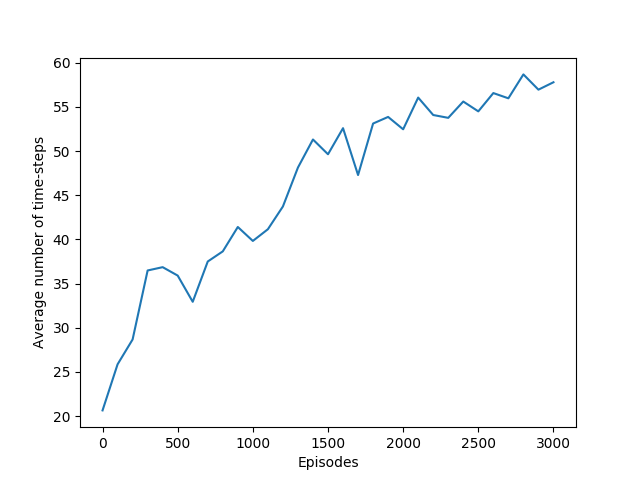
\includegraphics[scale=1]{part3a.png}
	\caption*{Changes of Time-steps per Episode}
\end{figure*}

The change of weights of the policy function are as follows:
\begingroup
\obeylines
\input{weight_change.txt}%
\endgroup%
\subsection*{Part 3(b)}
\paragraph{Question}
Explain why the final weights you obtained make sense. This requires understanding the what each input dimension means

\paragraph{Answer}

\begin{figure*}[h]
	\centering
	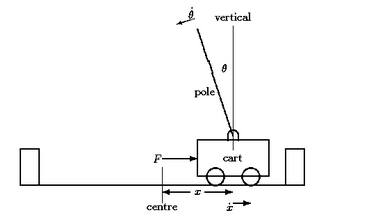
\includegraphics[scale=2.0]{cartpole_image.png}
	\caption*{Diagram representation of the cartpole system}
\end{figure*}

In order to understand why does the final weight make sense, we need to first understand what each input dimension means. The size of the input dimension is 4, which are [position of cart, velocity of cart, angle of pole, rotation rate (angular velocity) of pole]. In the source code, they are denoted by $[x, x\_dot, theta, theta\_dot]$ (dot means first derivative). Thus at each iteration when we observe the environment, we will observe the 4 components of the cart. The threshold for $x$ is 2.4 units away from the center, and the threshold for $theta$ is 15 degrees from the vertical.

When looking at the final weights, there are some observations that we made:
\begin {itemize}
	\item For velocity, angle, and angular velocity, the system tries to balance it using the weights. The weights for those components are approximately the same in magnitude but with different signs.
	\item For angular velocity, if it is is negative (falling to the left), $theta\_dot \times w_{theta\_dot_L}$ will be positive, while $theta\_dot \times w_{theta\_dot_R}$ will be negative. Thus it will want the cart to be pushed towards the left side (0) to reduce the angular velocity. On the other hand, if angular velocity is positive (falling to the right), it will want the cart to be pushed towards the right (1) to cancel out the momentum.
	\item Similarly for velocity, when the velocity of the cart is negative (moving to the left), $x\_dot \times w_{x\_dot_L}$ will be negative while $x\_dot \times w_{x\_dot_R}$ will be positive. Thus based on velocity, the cart will want to be pushed towards the right (1), vice versa. We want to keep the movement of the cart to minimum so there won't be too much force applied onto the pole.
	\item Same explanation goes for $theta$. The system would want to use the weight to keep the $theta$ to be approximately 0 (vertically upright).
	\item The trained system prioritize balancing velocity, angle, and angular velocity over the distance of cart. This can be observed because the system uses the weight to balance out the velocity, angle, and angular velocity (as described in point 1). However, the sign of $w_{x_L}$ and $w_{x_R}$ are the same, and unlike the other components, the magnitude is relatively not close. The potential reason for this can be because the system is not done training yet. We are only reaching an average step of 50 as supposed to reaching average reward of 195 over 100 consecutive trials.
	\item One minor observation is that the magnitude of $w_{x\_dot}$ and $w_{theta\_dot}$ are both bigger than magnitude of $w_x$ and $w_{theta}$ respectively. This make sense because when the system is calculating the new state of the cart given an action, the velocity's are multiplied with $\tau=0.02$, which is the time interval. Thus even though the magnitude of the weight is big, the resulting component would be smaller.
\end {itemize}

\clearpage



\end{document}